%!TEX output_directory=output

\documentclass[20pt,margin=1in,innermargin=-7in,blockverticalspace=-0in]{tikzposter}
\geometry{paperwidth=48in,paperheight=35in}

\usepackage{kaufman}
\usepackage{dartmouth-theme}

\addbibresource{../refs.bib}

% set theme parameters
\tikzposterlatexaffectionproofoff
\usetheme{DartmouthTheme}
\usecolorstyle{DartmouthStyle}

\title{Hamiltonian Engineering via Reinforcement Learning}
\author{Will Kaufman}
\institute{Dartmouth College}
\titlegraphic{\includegraphics[width=0.03\textwidth]{lonepine.pdf}}

% begin document
\begin{document}
\maketitle
\centering
\begin{columns}
    \column{0.33}
    
    \block{Hamiltonian engineering problem}{
    The time evolution of a quantum system depends on the system's Hamiltonian, a self-adjoint operator whose eigenvalues correspond to possible energy measurements. For a system with initial density operator $\rho(0)$ and Hamiltonian $H(t)$, the state at time $t$ is given by
    \[
    \rho(t) = U(t)\rho(0)U^\dagger(t)
    \]
    where the propagator $U(t)$ is defined by
    \begin{equation}
        i\hbar \ddt{U(t)} = H(t) U(t), U(0) = \identity
    \end{equation}
    The total Hamiltonian $H(t)$ can generally be broken into a time-independent system Hamiltonian and a time-dependent control Hamiltonian
    \begin{equation}
        H(t) = H_\text{system} + H_\text{control}(t)
    \end{equation}
    Hamiltonian engineering seeks to design the time-dependent Hamiltonian $H_\text{control}(t)$ to control the system's evolution so that it appears to evolve under a target ``effective'' Hamiltonian ($H_\text{target}$) when measured stroboscopically. That is,
    \begin{equation}\label{eq:strob_measure}
        \rho(Nt_c) = U_\text{target}(Nt_c) \rho(0) U_\text{target}^\dagger(Nt_c)
    \end{equation}
    where $U_\text{target}$ is the propagator determined by $H_\text{target}$, $t_c$ is the cycle time, and $N \in \N$. If $H(t)$ determines the propagator $U(t)$, then equation~\ref{eq:strob_measure} is implied by
    \begin{equation}\label{eq:ham_engineering}
        U(Nt_c) = U_\text{target}(Nt_c)
    \end{equation}
    } % end hamiltonian engineering problem block
    
    \block{Average Hamiltonian theory}{
    Average Hamiltonian theory is one approach to solving the Hamiltonian engineering problem
    \cite{PhysRev.175.453}
    . For a system of spins in a magnetic field, the internal Hamiltonian contains a chemical shift term and a dipolar coupling term
    \begin{equation}\label{eq:ham_spin}
        H_\text{int} = \sum_i \delta_i I_z^{(i)} + \sum_{i,j} d_{ij} \left( 3I_z^{(i)}I_z^{(j)} - \mathbf{I^{(i)}} \cdot \mathbf{I^{(j)}} \right) = H_\text{CS} + H_\text{D}
    \end{equation}
    Applying a magnetic field pulse along the transverse axis performs a global rotation of the spins. The magnetic field pulses manifest themselves as a time-dependent interaction $H_\text{rf}(t)$.
    If a pulse sequence with cycle time is both cyclic and periodic
    \cite{gerstein-dybowski}
    \begin{align}\label{eq:AHT_conditions}
        U_\text{rf}(t_c) &= T\exp \left(
            -i/\hbar \int_0^{t_c} H_\text{rf}(t) dt \right) = \pm \identity
            & \text{(cyclic)} \\
        H_\text{rf}(t) &= H_\text{rf}(t + Nt_c) & \text{(periodic)}
    \end{align}
    then, using the Magnus Expansion, the propagator can be given by
    \begin{align}\label{eq:AHT_average}
        U(t_c) &= \exp\left( \frac{-i}{\hbar} t_c (\overline{H}^{(0)} +
            \overline{H}^{(1)} + \dots) \right) \\
        \overline{H}^{(0)} &= 1/t_c \int_0^{t_c}
            U_\text{rf}(t) H_\text{int} U_\text{rf}^\dagger(t) dt
    \end{align}
    To engineer a target Hamiltonian $H_t$, the pulse sequence is chosen so that $\overline{H}^{(0)} = H_t$.
    
    Several pulse sequences have been developed using the average Hamiltonian theory framework \cite{PhysRevLett.20.180, PhysRevLett.119.183603, O_Keeffe_2019}.
    For example, the WAHUHA 4-pulse sequence applied to a spin system with $H_\text{int}$ given in eq~\ref{eq:ham_spin} has the zeroth-order average Hamiltonian $\overline{H}^{(0)} = \frac{1}{3} \sum_i \delta_i \left( I_x^{(i)} + I_y^{(i)} + I_z^{(i)} \right)$.
    
    Average Hamiltonian theory assumes that higher-order terms in the Magnus Expansion (eq~\ref{eq:AHT_average}) are negligible. This is often true in the regime where $t_c |H_\text{int}| \ll 1$, but $t_c$ is constrained by experimental limitations in the accuracy of pulse timings and strengths.
    } % end AHT block
    
    \block{Reinforcement learning}{
    Reinforcement learning (RL) is being investigated as an alternative approach to Hamiltonian engineering for spin systems.
    ``Reinforcement learning is learning what to do--how to map situations to actions--so as to maximize a numerical reward signal'' \cite{sutton2018reinforcement}. RL has been applied to a variety of different problems, including playing games such as chess or Go \cite{Silver1140} and interacting with physical environments such as balancing a pole \cite{lillicrap2015continuous}.
    } % end rl block
    
    \column{0.33}
    
    \block{Reinforcement learning (cont.)}{
    
    The RL paradigm involves an \emph{agent} that makes observations on the \emph{state} of the \emph{environment}, performs \emph{actions} on the environment, and receives \emph{rewards} based on its performance (see figure~\ref{fig:RL}).
    
    \begin{minipage}{\linewidth}
    \begin{figure}[H]
        \centering
        \scalebox{1.5}{
        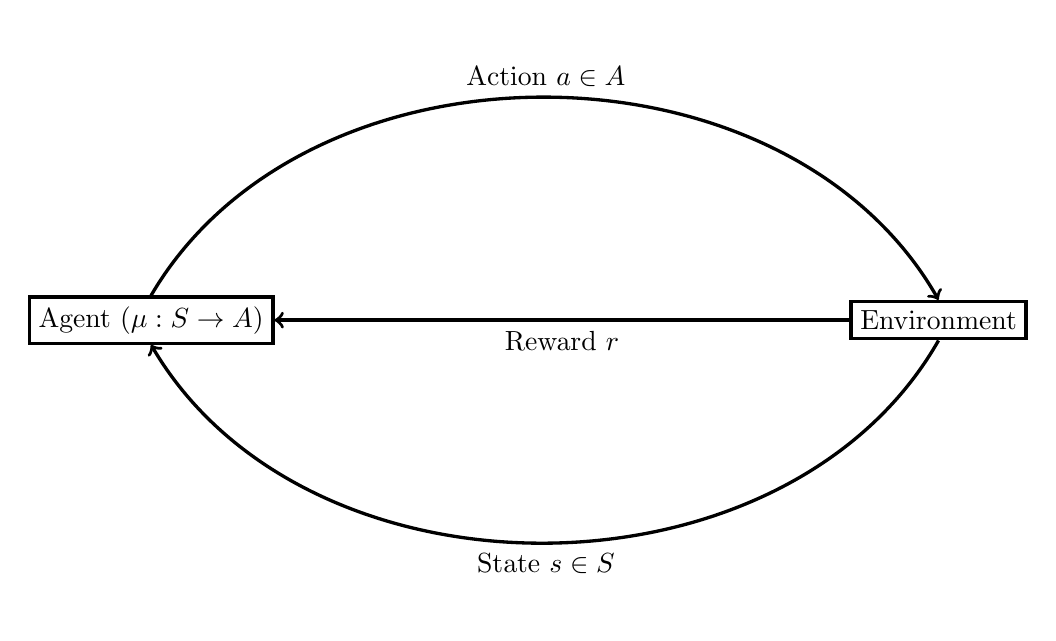
\begin{tikzpicture}[->, very thick]
             %nodes
             \node[draw] at (-5,0) (agent) {Agent ($\mu: S \to A$)};
             \node[draw] at (5,0) (env) {Environment};
             \path
                 (agent.north) edge[bend left=60] node[above] {Action $a \in A$} (env.north)
                 (env.south) edge[bend left=60] node[below] {State $s \in S$} (agent.south)
                 (env.west) edge node[below] {Reward $r$} (agent.east);
        \end{tikzpicture}
        }
        \caption{The general reinforcement learning paradigm.}
        \label{fig:RL}
    \end{figure}
    \end{minipage}
    The agent learns a policy function $\mu:S\to A$ which maps a given state to the action that will lead to the largest rewards. In many RL algorithms, an action-value function $Q_\mu(s,a)$ is also learned. The action-value function gives the expected total rewards by performing action $a$ when in state $s$, then following $\mu$.
    
    Several algorithms have been developed for various realizations of the RL problem. Deep deterministic policy gradient (DDPG) uses neural networks to approximate the policy $\mu(s|\theta_\mu)$ and the action-value function $Q(s,a|\theta_Q)$ for continuous action spaces \cite{lillicrap2015continuous}.
    % TODO include specifically how training works?
    Both $\mu$ and $Q$ are trained using gradient-based methods. $Q$ is optimized by minimizing the loss function
    \begin{equation}\label{eq:critic_loss}
        L(\theta_Q) = \E\left[ (Q(s,a|\theta_Q) - y_t)^2 \right]
    \end{equation}
    where
    \[
    y_t = r(s,a) + \gamma Q(s', \mu(s')|theta_Q)
    \]
    $s'$ is the state after performing action $a$.
    The policy $\mu$ is optimized by maximizing the performance $J$ (generally taken to be the action-value function $Q$) via gradient ascent
    \begin{equation}\label{eq:actor_train}
        \nabla_{\theta_\mu} J = \E\left[
            \nabla_{\theta_\mu} Q(s,\mu(s|\theta_\mu))
        \right]
    \end{equation}
    The gradients are estimated from a random subset of experiences $(s,a,r,s')$.
    
    In \cite{khadka2018evolutionguided}, a hybrid algorithm called Evolutionary Reinforcement Learning (ERL) uses both DDPG and genetic algorithms to prevent premature convergence to local optima and speed up learning. In ERL, a population of policy functions are maintained, as well as gradient-based policy and action-value functions. A diagram of the algorithm is presented in figure~\ref{fig:ERL}.
    \begin{minipage}{\linewidth}
    \begin{figure}[H]
        \centering
        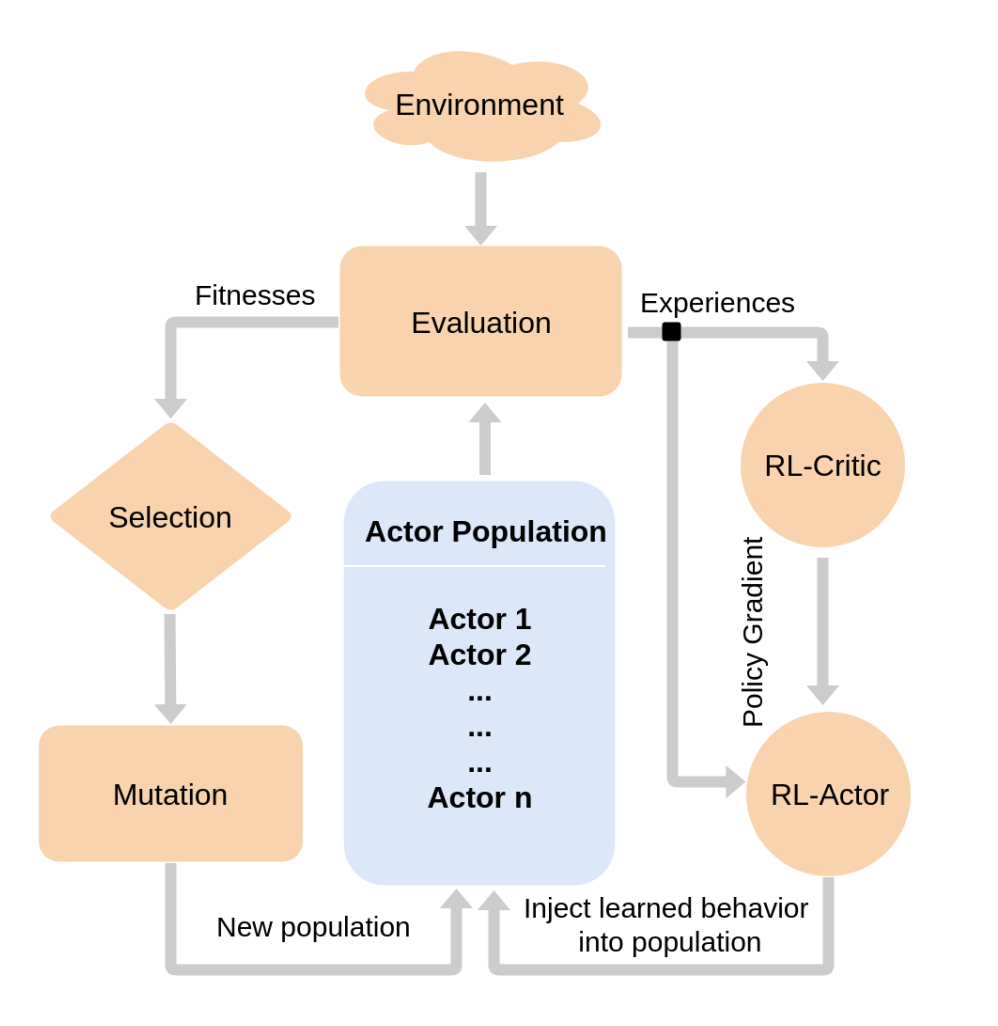
\includegraphics[width=0.7\linewidth]{graphics/ERL.png}
        \caption{The general overview of the ERL algorithm, reproduced from \cite{khadka2018evolutionguided}.}
        \label{fig:ERL}
    \end{figure}
    \end{minipage}
    % TODO conclusion sentence?
    } % end RL block
    
    \column{0.33}
    
    \block{Applying RL to Hamiltonian engineering}{
    In the case of Hamiltonian engineering, the states correspond to the propagators of the system at different times, the actions correspond to pulses or delays, and the reward signal quantifies the degree to which the system has evolved under the target effective Hamiltonian.
    The fidelity of two unitary operators can be quantified by
    \begin{equation}\label{eq:fidelity}
        \text{fidelity}(U_\text{target}^\dagger, U) = \left| \text{Tr}\left( \frac{U_\text{target}^\dagger U}{2^N} \right) \right|
    \end{equation}
    and takes on values between $0$ and $1$, where $1$ implies the two unitary operators are equal.
    Using this definition of fidelity, the rewards in the RL algorithm are
    \begin{equation}\label{eq:rewards}
        r = -\log\left( 1- \text{fidelity}(U_\text{target}, U_\text{exp})^{\tau/t} \right)
    \end{equation}
    The exponent $\tau/t$ makes rewards comparable across different duration pulses sequences.
    
    The actions are magnetic field pulses that perform global rotations, and can therefore be parametrized by the axis of rotation, the rotation angle $\alpha$, and the time $dt$ over which the rotation is performed.
    The axis of rotation is assumed to lie in the xy-plane, so a single pulse can be characterized by the tuple $(\phi, \alpha, dt) \in [-\pi,\pi] \times [-\alpha_\text{max}, \alpha_\text{max}] \times [t_\text{min}, \inf)$.
    The state is represented by the sequence of all previous actions performed.
    The state and actions are represented by values in the interval $[-1,1]$ according to the following map
    \begin{align}
        \phi \in [-\pi, \pi], \phi      &\mapsto \phi / \pi \\
        \alpha \in [-2\pi,2\pi],\alpha  &\mapsto \alpha / 2\pi \\
        t \in [0,5\cdot10^{-6}], t      &\mapsto
            \frac{\log_{10}(t + 10^{-7}) + 7}{0.853785} - 1
    \end{align}
    This encoding of action and state representations is necessary for the training and stability of the neural networks.
    
    % TODO include diagram of NN architecture?
    
    } % end application section
    
    
    \block{Results and further work}{
    
    Applying ERL to Hamiltonian engineering has so far been unsuccessful. Neither the gradient-based nor population policy functions have consistently achieved rewards above $3$, which corresponds to a fidelity of $0.999$. For experimental applications, this is far too low a fidelity to be useful. The poor performance may be due to poor choice of hyperparameters (such as the learning rate or the number of observations from which to learn) or ineffective exploration of both state and action space.
    
    In addition to varying hyperparameters or changing the noise processes used in ERL, reformulating the problem in terms of discrete actions (i.e. only performing $\pi/2$ rotations along the $x$ or $y$ axis) could be promising. This has generally been the approach within the average Hamiltonian theory framework, as well as with preliminary investigations into reinforcement learning for Hamiltonian engineering.
    % TODO how to cite Pai/Xiao?
    Finally, including experimental errors or constraints, such as phase errors or finite pulse widths, would more accurately reflect the pulse sequence performances.
    } % end further work
    
    \block{References}{
    \printbibliography[heading=none]
    }
\end{columns}
\end{document}
